\title{Change of Variable}
\subtitle{\SubTitleName}
\institute[]{\Course}
\author{\Instructor}
\maketitle   
  



\frame{\frametitle{Topics and Objectives}
    \Emph{Topics} \\
    %\TopicStatement
    \begin{itemize}
    
        % \item representing quadratic forms with symmetric matrices
        \item change of variables
        \item principle axes theorem
        % \item Classifying quadratic forms
    
    \end{itemize}
    
    \vspace{0.5cm}
    
    \Emph{Learning Objectives}\\
    
    %\LearningObjectiveStatement
    
    \begin{itemize}
    
        % \item characterize and classify quadratic forms using eigenvalues and eigenvectors
        % \item express quadratic forms in the form $Q (\vec x ) =  \vec x ^{\, T} A \vec x$
        \item apply the principle axes theorem to express quadratic forms with no cross-product terms.
        
    \end{itemize}
    
    \vspace{0.25cm} 
    


} 



\begin{frame}{A Motivating Question}

    Does this inequality hold for all $x,y$?  
    \begin{equation*}
        x^2 - 6 xy + 9 y ^2 \geq 0
    \end{equation*}
    \onslide<2->{To answer this question, consider the following. }
    \begin{itemize}
        \item<2-> The polynomial $Q= x^2 - 6 xy + 9 y ^2$ is an example of a quadratic form. 
        \item<3-> The $-6xy$ term is a \Emph{cross-product} term because it contains both variables. 
        \item<4-> The cross-product term makes problems like this one more complicated. 
        \item<5-> What can we do to simplify our problem? 
    \end{itemize}
    
\end{frame}




\begin{frame}\frametitle{Change of Variable}

    Given $Q=\vec x\,^T A\vec x$, where $\vec x \in \mathbb R^n$ is a variable vector and $A$ is a real $n\times n$ symmetric matrix. Then, $$A = PDP^T$$ where $P$ is an $n \times n$ orthogonal matrix. \onslide<2->{ A \Emph{change of variable} can be represented as $$\vec x = P\vec y, \quad \mathrm{or} \quad \vec y = P^{-1}\vec x$$}
    \onslide<3->{With this change of variable, the quadratic form $\vec x \,^T A\vec x$ becomes:}
    \begin{align*}
        \onslide<4->{Q = \vec x \,^T A\vec x &= (P\vec y)^T A (P\vec y) \\}
        \onslide<5->{ &= \vec y\, ^T P^T A P\vec y \\}
        \onslide<6->{ &= \vec y\, ^T D\vec y , \quad \text{using } A = PDP^T}
    \end{align*}
    \onslide<7->{Thus, $Q$ is expressed without cross-product terms. }
\end{frame}

\begin{frame}\frametitle{Principle Axes Theorem}

    \begin{center}\begin{tikzpicture} \node [mybox](box){\begin{minipage}{0.95\textwidth}\vspace{2pt}
        If $A$ is a symmetric matrix then there exists an orthogonal change of variable $\vec x = P \vec y$ that transforms $\vec x^{\,T} A \vec x$ to $\vec y^{\,T} D \vec y$ with no cross-product terms. 
    \end{minipage}};
    \node[fancytitle, right=10pt] at (box.north west) {Theorem};
    \end{tikzpicture}\end{center}
    \pause 
    \textit{Proof on previous slide. }
    

\end{frame}




\begin{frame}\frametitle{Example}
    
    Compute the quadratic form $Q = \vec x^{\,T} A \vec x$ for $A = \spalignmat{5 2;2 8}$, and identify a change of variable that removes the cross-product term. The eigenvalues and eigenvectors of $A$ are given below. 
    $$\lambda_1 = 9, \quad \lambda_2 = 4, \quad \vec v_1 = \spalignmat{2;-1}, \quad \vec v_2 = \spalignmat{1;2}$$
    \pause
    \Emph{Solution}\\
    Our change of variable is $$\vec x = P \vec y, \quad P = \frac{1}{\sqrt5}\spalignmat{2 1;-1 2}$$
    Using this change of variable,
    $Q = \vec x\, ^TA\vec x = \vec y\, ^T D \vec y = 9y_1^2 + 4y_2^2$.
\end{frame}


\begin{frame}\frametitle{Example}
    If, for example, we set $Q=1$, we obtain two curves. 
    \vspace{-12pt}
    \begin{columns}
    \begin{column}{.35\textwidth}
    \begin{center}
        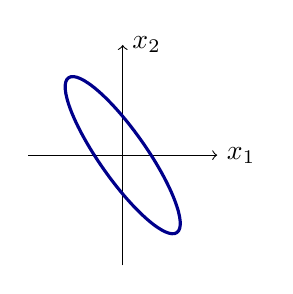
\begin{tikzpicture}[scale=0.4]
            \onslide<2->{\draw[->] (-3,0) -- (3,0) node[right] {$x_1$};
            \draw[->] (0,-3.5) -- (0,3.5) node[right] {$x_2$};
            \draw[rotate=35, DarkBlue, line width = 0.4mm] (0, 0) ellipse (.75cm and 3cm);}
        \end{tikzpicture}    \onslide<2->{$Q = 5x^2+4xy+8y^2= 1$ } \end{center}
    \end{column}\begin{column}{.35\textwidth}\begin{center}
        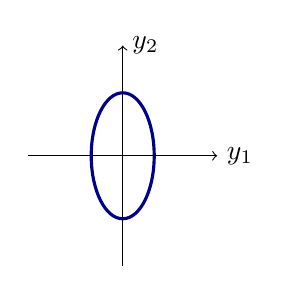
\begin{tikzpicture}[scale=0.4]
        \onslide<3->{
            \draw[->] (-3,0) -- (3,0) node[right] {$y_1$};
            \draw[->] (0,-3.5) -- (0,3.5) node[right] {$y_2$};
            \draw[rotate=0, DarkBlue, line width = 0.4mm] (0, 0) ellipse (1cm and 2cm);}
        \end{tikzpicture}        \onslide<3->{$Q = 9y_1^2 + 4y_2^2 = 1 $}         \end{center}
    \end{column}
    \end{columns} 
    \vspace{18pt}
    \onslide<4->{
    Using our change of variable, we can more easily }
    \begin{itemize}
        \item<5-> identify points on the ellipse that are closest/furthest from the origin
        \item<6-> determine whether $Q$ can take on negative/positive values
    \end{itemize}
    
    
\end{frame}





\begin{frame}\frametitle{Inequality Example}

    We can now return to our motivating question (from first slide): does this inequality hold for all $x,y$?  
    \begin{equation*}
        x^2 - 6 xy + 9 y ^2 \geq 0
    \end{equation*}
    \pause 
    \Emph{Solution}
    
    Set $Q = x^2 - 6 xy + 9 y ^2$, then 
    \pause 
    \begin{align*}
        Q &= x^2 - 6 xy + 9 y ^2 = \vec x\, ^T \spalignmat{1 -3;-3 9}\vec x , \quad A = \spalignmat{1 -3;-3 9} 
    \end{align*}
    \pause 
    By inspection, $A$ is singular $ \Rightarrow \lambda_1 = 0$.\pause The sum of the eigenvalues is the trace $\Rightarrow \lambda_2 = 10$. \pause $$Q = \vec y \, ^T D \vec y = 0y_1^2 + 10 y_2^2$$
    \pause $Q$ can be zero but is never negative. The inequality holds. 
\end{frame}




\frame{\frametitle{Summary}

    \SummaryLine \vspace{4pt}
    \begin{itemize}\setlength{\itemsep}{8pt}

        \item the representation of quadratic forms with symmetric matrices
        \item a change of variable to represent quadratic forms without cross-product terms
        \item the Principle Axis Theorem

    \end{itemize}
    
    \vspace{6pt}

    We saw how we can express quadratic forms in the form $Q (\vec x ) =  \vec x ^{\, T} A \vec x$, for $\vec x \in \mathbb R^n$ without cross-product terms. 
    \pause
    
}




% \begin{frame}\frametitle{Example 3}
%     Make a change of variable $\vec x = P \vec y$ that transforms $Q = \vec x^T A \vec x$ so that it does not have cross terms. The orthogonal decomposition of $A$ is given. 
%     \begin{align*} 
%         A &= \spalignmat{3 2;2 6} = PDP^T , \quad 
%         P = \frac{1}{\sqrt 5}\spalignmat{2 1;-1 2}, \quad 
%         D = \spalignmat{2 0;0 7}
%     \end{align*}
    


% \end{frame}





%\begin{frame}\frametitle{Example 4}
%
%    \vspace{-24pt} 
%    
%    \begin{columns}
%    \begin{column}{.4\textwidth}
%    \begin{center}
%        \begin{tikzpicture}[scale=0.95]
%            \draw[->] (-2,0) -- (2,0) node[right] {$x_1$};
%            \draw[->] (0,-2) -- (0,2) node[above] {$x_2$};
%            \draw [rotate=0,blue,thick] (0,0) ellipse (20pt and 30pt);  
%        \end{tikzpicture}
%    \end{center}
%    \end{column}
%    \begin{column}{.6\textwidth}
%        \vskip .25cm
%        Suppose $A = \spalignmat{9 0;0 4}$. How are the eigenvectors of $A$ related to the curve             $C = \vec x^{\,T} \spalignmat{9 0;0 4} \vec x$ ? 
%    \end{column}
%    \end{columns}
%    
%\end{frame}